% Options for packages loaded elsewhere
\PassOptionsToPackage{unicode}{hyperref}
\PassOptionsToPackage{hyphens}{url}
%
\documentclass[
]{article}
\usepackage{lmodern}
\usepackage{amssymb,amsmath}
\usepackage{ifxetex,ifluatex}
\ifnum 0\ifxetex 1\fi\ifluatex 1\fi=0 % if pdftex
  \usepackage[T1]{fontenc}
  \usepackage[utf8]{inputenc}
  \usepackage{textcomp} % provide euro and other symbols
\else % if luatex or xetex
  \usepackage{unicode-math}
  \defaultfontfeatures{Scale=MatchLowercase}
  \defaultfontfeatures[\rmfamily]{Ligatures=TeX,Scale=1}
\fi
% Use upquote if available, for straight quotes in verbatim environments
\IfFileExists{upquote.sty}{\usepackage{upquote}}{}
\IfFileExists{microtype.sty}{% use microtype if available
  \usepackage[]{microtype}
  \UseMicrotypeSet[protrusion]{basicmath} % disable protrusion for tt fonts
}{}
\makeatletter
\@ifundefined{KOMAClassName}{% if non-KOMA class
  \IfFileExists{parskip.sty}{%
    \usepackage{parskip}
  }{% else
    \setlength{\parindent}{0pt}
    \setlength{\parskip}{6pt plus 2pt minus 1pt}}
}{% if KOMA class
  \KOMAoptions{parskip=half}}
\makeatother
\usepackage{xcolor}
\IfFileExists{xurl.sty}{\usepackage{xurl}}{} % add URL line breaks if available
\IfFileExists{bookmark.sty}{\usepackage{bookmark}}{\usepackage{hyperref}}
\hypersetup{
  pdftitle={Laura\_SKF\_GoNoGo\_ErrorTrialsAnalsysis},
  pdfauthor={Marios Panayi},
  hidelinks,
  pdfcreator={LaTeX via pandoc}}
\urlstyle{same} % disable monospaced font for URLs
\usepackage[margin=1in]{geometry}
\usepackage{graphicx,grffile}
\makeatletter
\def\maxwidth{\ifdim\Gin@nat@width>\linewidth\linewidth\else\Gin@nat@width\fi}
\def\maxheight{\ifdim\Gin@nat@height>\textheight\textheight\else\Gin@nat@height\fi}
\makeatother
% Scale images if necessary, so that they will not overflow the page
% margins by default, and it is still possible to overwrite the defaults
% using explicit options in \includegraphics[width, height, ...]{}
\setkeys{Gin}{width=\maxwidth,height=\maxheight,keepaspectratio}
% Set default figure placement to htbp
\makeatletter
\def\fps@figure{htbp}
\makeatother
\setlength{\emergencystretch}{3em} % prevent overfull lines
\providecommand{\tightlist}{%
  \setlength{\itemsep}{0pt}\setlength{\parskip}{0pt}}
\setcounter{secnumdepth}{-\maxdimen} % remove section numbering

\title{Laura\_SKF\_GoNoGo\_ErrorTrialsAnalsysis}
\author{Marios Panayi}
\date{1/27/2021}

\begin{document}
\maketitle

\begin{figure}
\centering
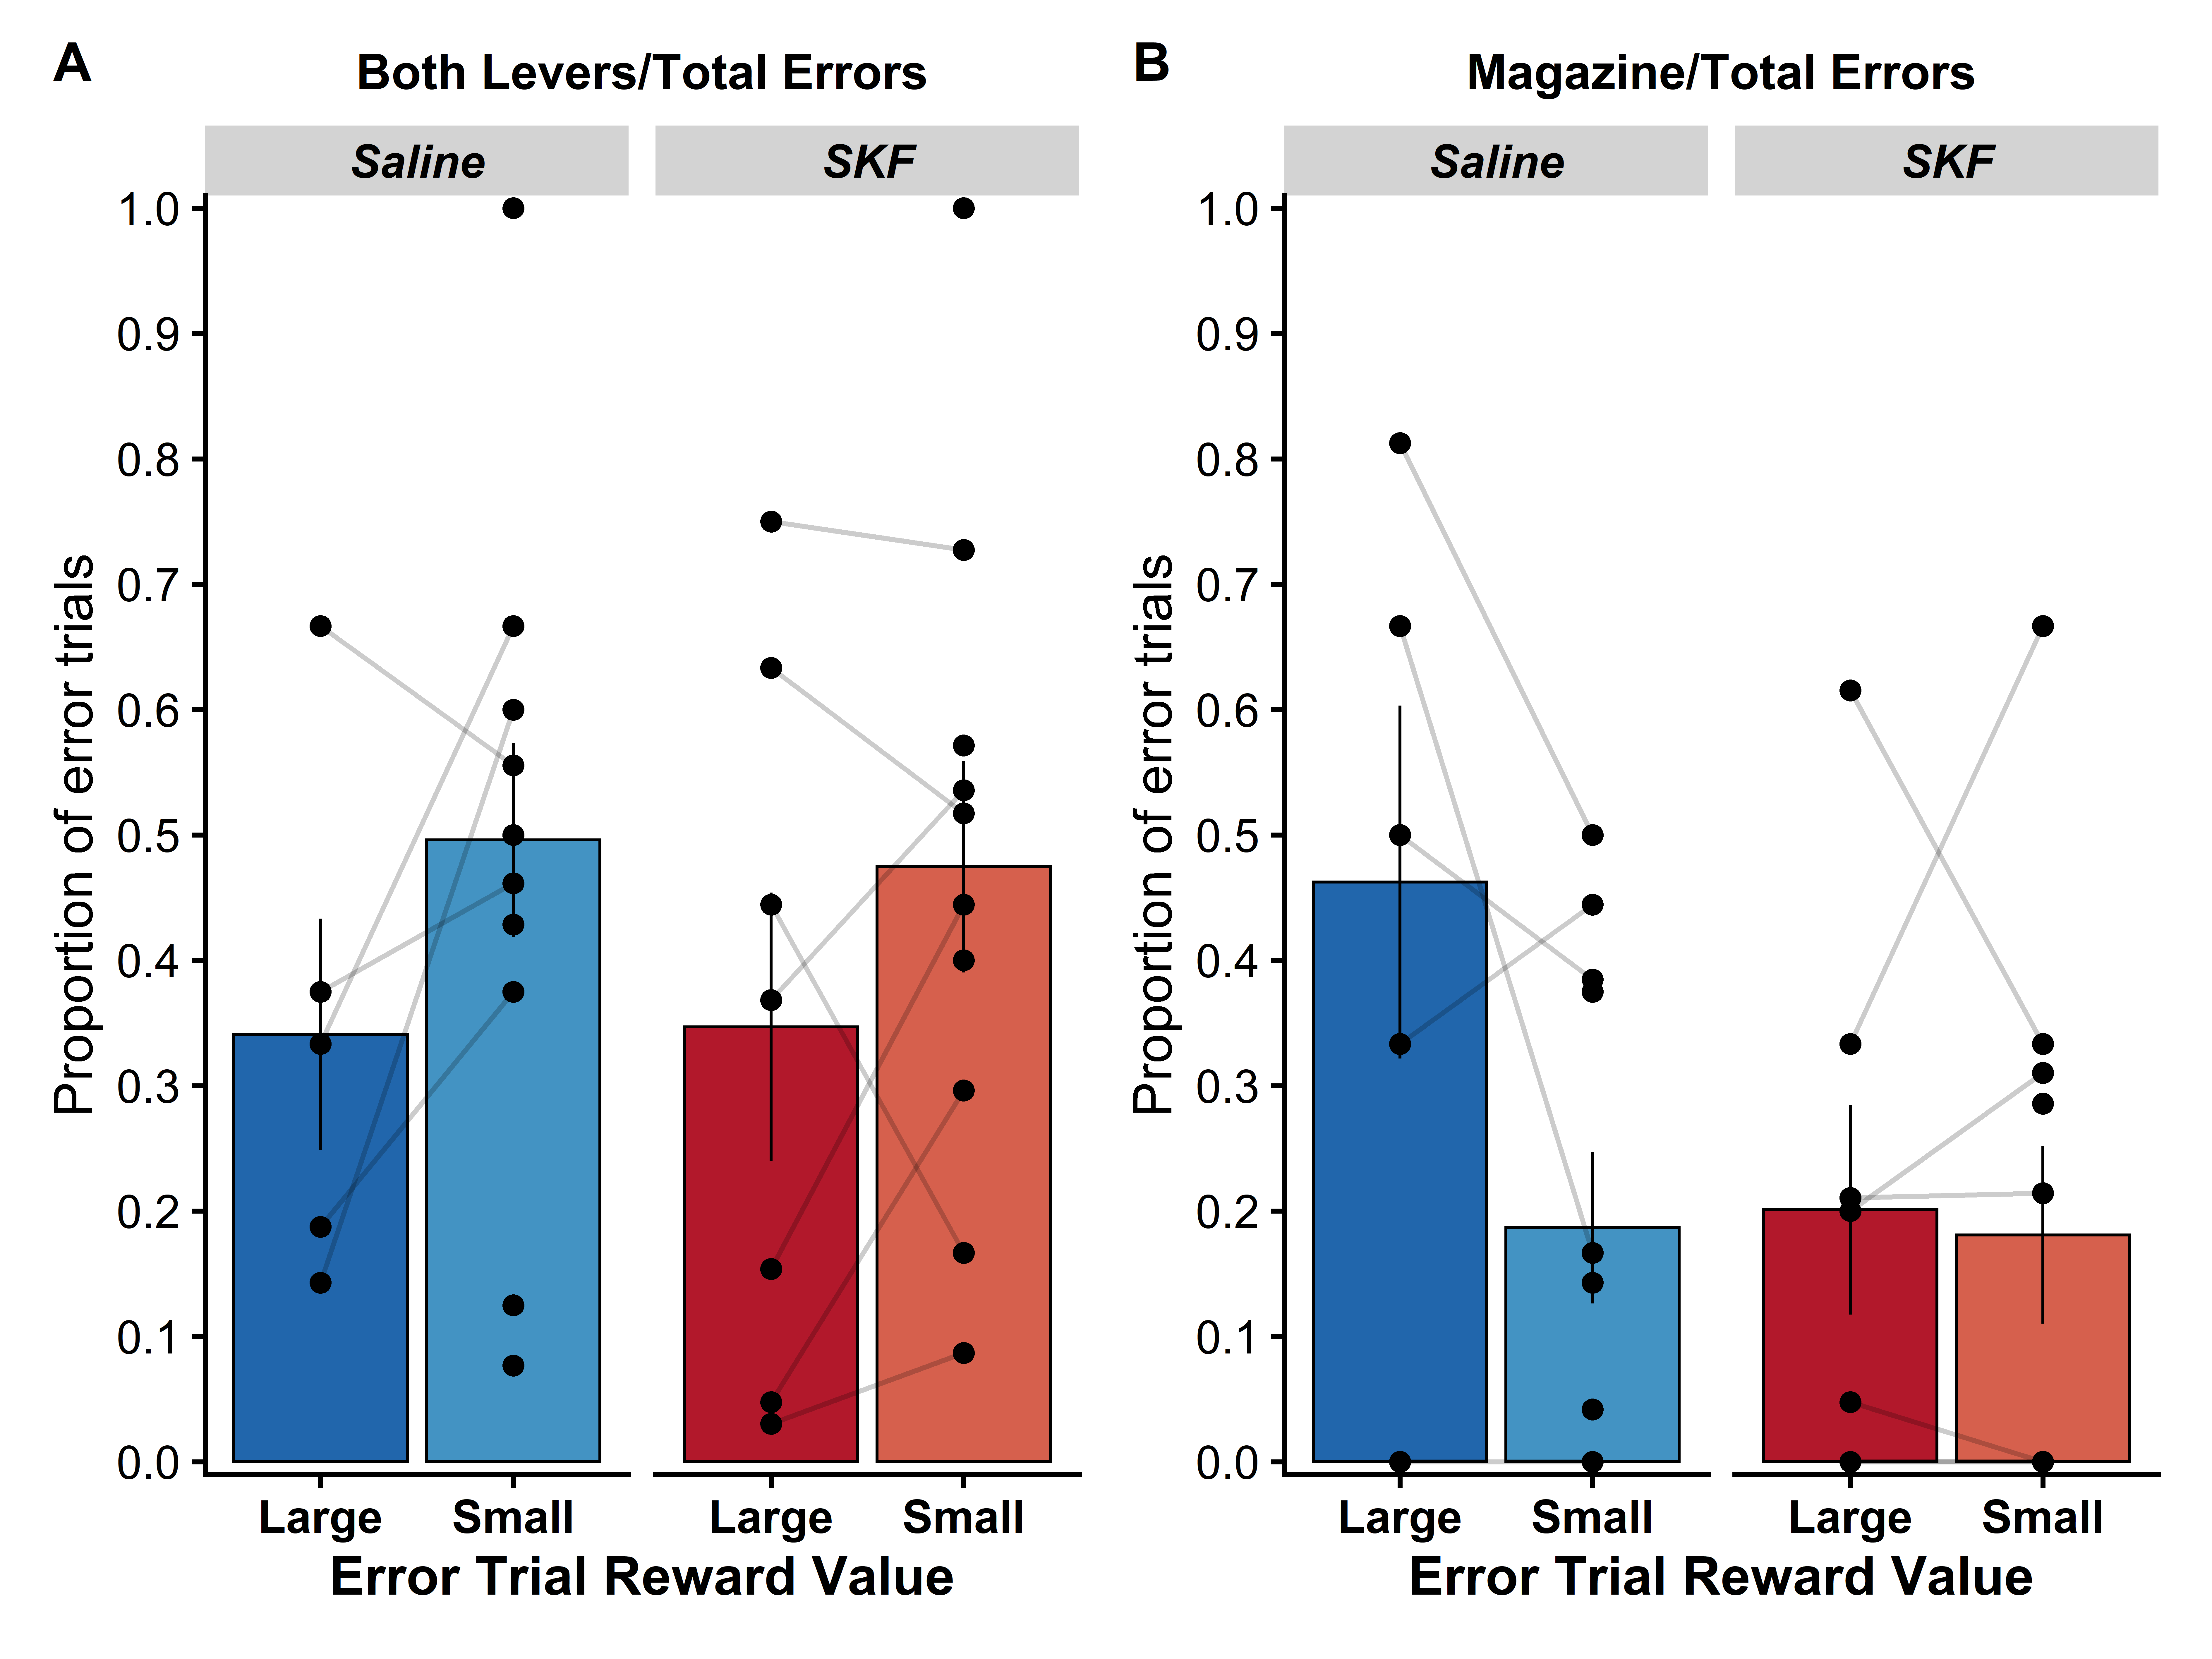
\includegraphics{../figures/Plots_LeversAndMag.png}
\caption{Probability of both levers or magazine}
\end{figure}

\hypertarget{a-analysis-of-both-levers-data}{%
\subsection{A) Analysis of both levers
data}\label{a-analysis-of-both-levers-data}}

\begin{table}[tbp]

\begin{center}
\begin{threeparttable}

\caption{\label{tab:Analysis 2: Probability of both levers }}

\begin{tabular}{lllll}
\toprule
 & \multicolumn{1}{c}{Df} & \multicolumn{1}{c}{Chisq} & \multicolumn{1}{c}{Chi Df} & \multicolumn{1}{c}{Pr(>Chisq)}\\
\midrule
RewardSize & 9.00 & 5.30 & 1.00 & 0.02\\
Drug & 9.00 & 1.10 & 1.00 & 0.29\\
RewardSize:Drug & 9.00 & 0.58 & 1.00 & 0.44\\
\bottomrule
\end{tabular}

\end{threeparttable}
\end{center}

\end{table}

\hypertarget{b-analysis-of-magazine-data}{%
\subsection{B) Analysis of magazine
data}\label{b-analysis-of-magazine-data}}

\begin{table}[tbp]

\begin{center}
\begin{threeparttable}

\caption{\label{tab:Analysis 2: Probability of both levers }}

\begin{tabular}{lllll}
\toprule
 & \multicolumn{1}{c}{Df} & \multicolumn{1}{c}{Chisq} & \multicolumn{1}{c}{Chi Df} & \multicolumn{1}{c}{Pr(>Chisq)}\\
\midrule
RewardSize & 9.00 & 0.66 & 1.00 & 0.42\\
Drug & 9.00 & 0.16 & 1.00 & 0.69\\
RewardSize:Drug & 9.00 & 1.03 & 1.00 & 0.31\\
\bottomrule
\end{tabular}

\end{threeparttable}
\end{center}

\end{table}

\begin{figure}
\centering
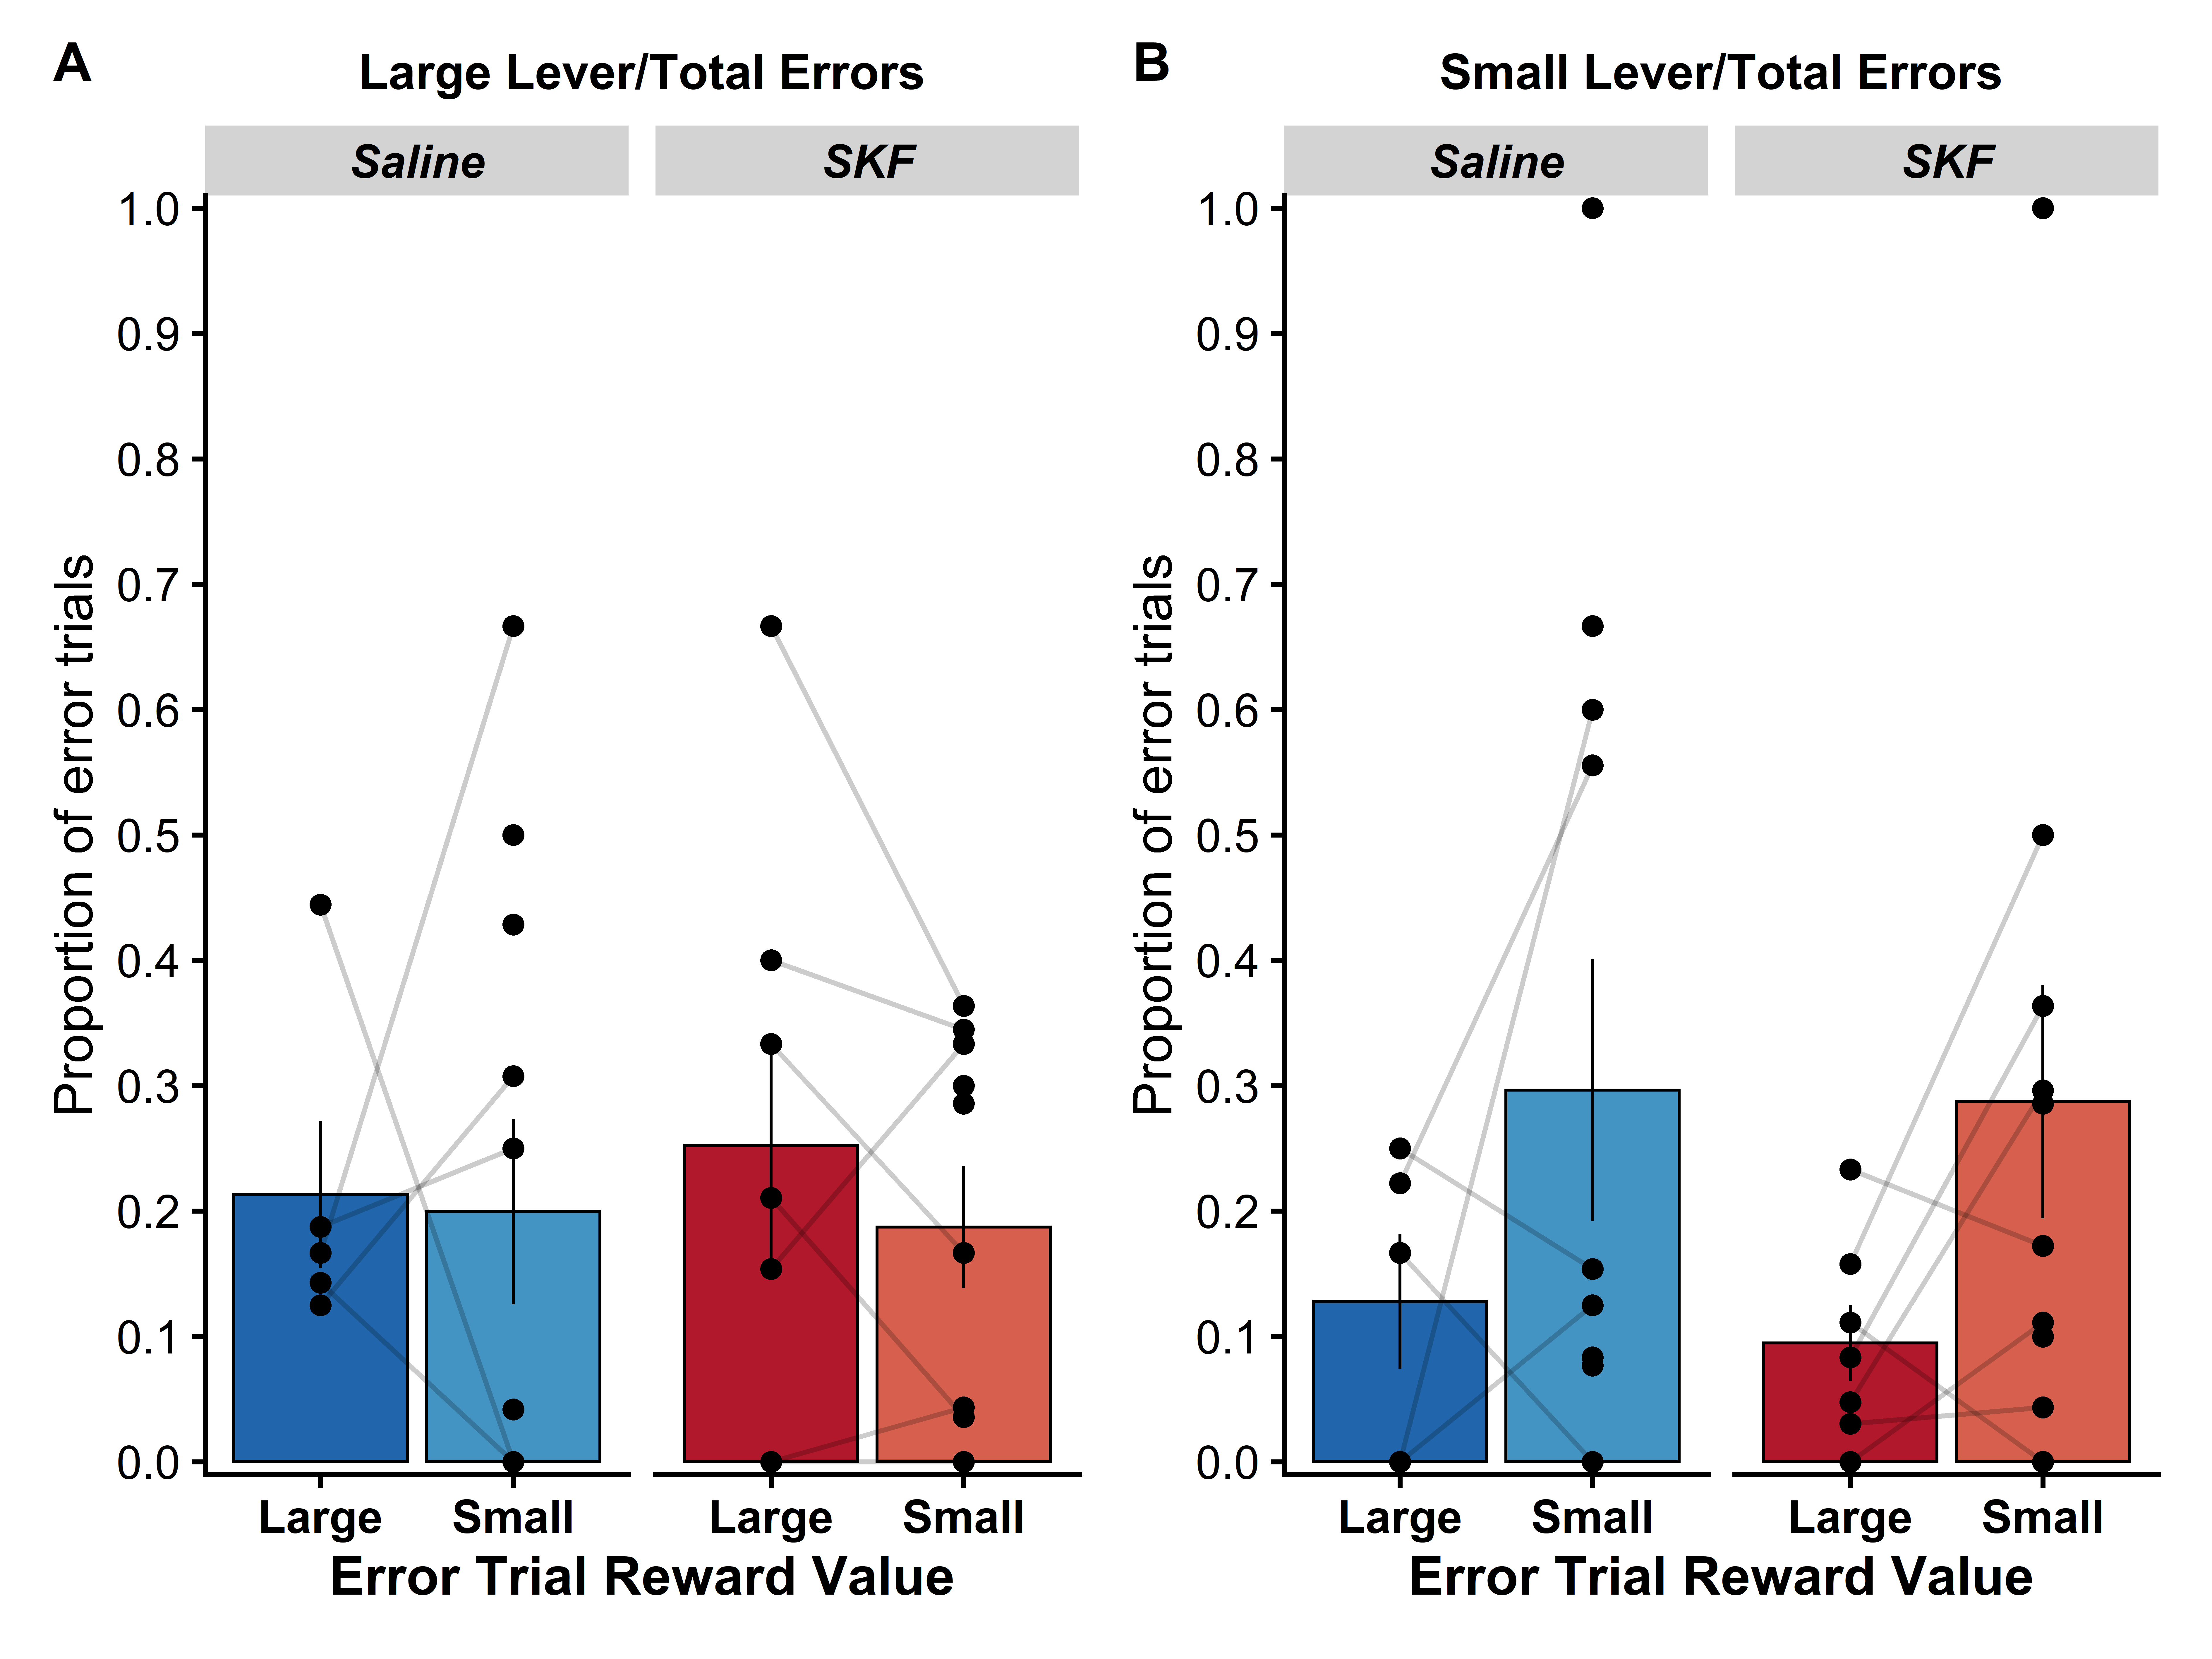
\includegraphics{../figures/Plots_LeversLargeVsSmall.png}
\caption{Probability of large and small reward levers}
\end{figure}

\hypertarget{a-analysis-of-large-reward-lever}{%
\subsection{A) Analysis of large reward
lever}\label{a-analysis-of-large-reward-lever}}

\begin{table}[tbp]

\begin{center}
\begin{threeparttable}

\caption{\label{tab:Analysis 2: Probability of both levers }}

\begin{tabular}{lllll}
\toprule
 & \multicolumn{1}{c}{Df} & \multicolumn{1}{c}{Chisq} & \multicolumn{1}{c}{Chi Df} & \multicolumn{1}{c}{Pr(>Chisq)}\\
\midrule
RewardSize & 9.00 & 0.39 & 1.00 & 0.53\\
Drug & 9.00 & 0.62 & 1.00 & 0.43\\
RewardSize:Drug & 9.00 & 0.06 & 1.00 & 0.81\\
\bottomrule
\end{tabular}

\end{threeparttable}
\end{center}

\end{table}

\hypertarget{b-analysis-of-large-reward-lever}{%
\subsection{B) Analysis of large reward
lever}\label{b-analysis-of-large-reward-lever}}

\begin{table}[tbp]

\begin{center}
\begin{threeparttable}

\caption{\label{tab:Analysis 2: Probability of both levers }}

\begin{tabular}{lllll}
\toprule
 & \multicolumn{1}{c}{Df} & \multicolumn{1}{c}{Chisq} & \multicolumn{1}{c}{Chi Df} & \multicolumn{1}{c}{Pr(>Chisq)}\\
\midrule
RewardSize & 9.00 & 7.93 & 1.00 & 0.00\\
Drug & 9.00 & 2.12 & 1.00 & 0.15\\
RewardSize:Drug & 9.00 & 0.18 & 1.00 & 0.67\\
\bottomrule
\end{tabular}

\end{threeparttable}
\end{center}

\end{table}

\begin{figure}
\centering
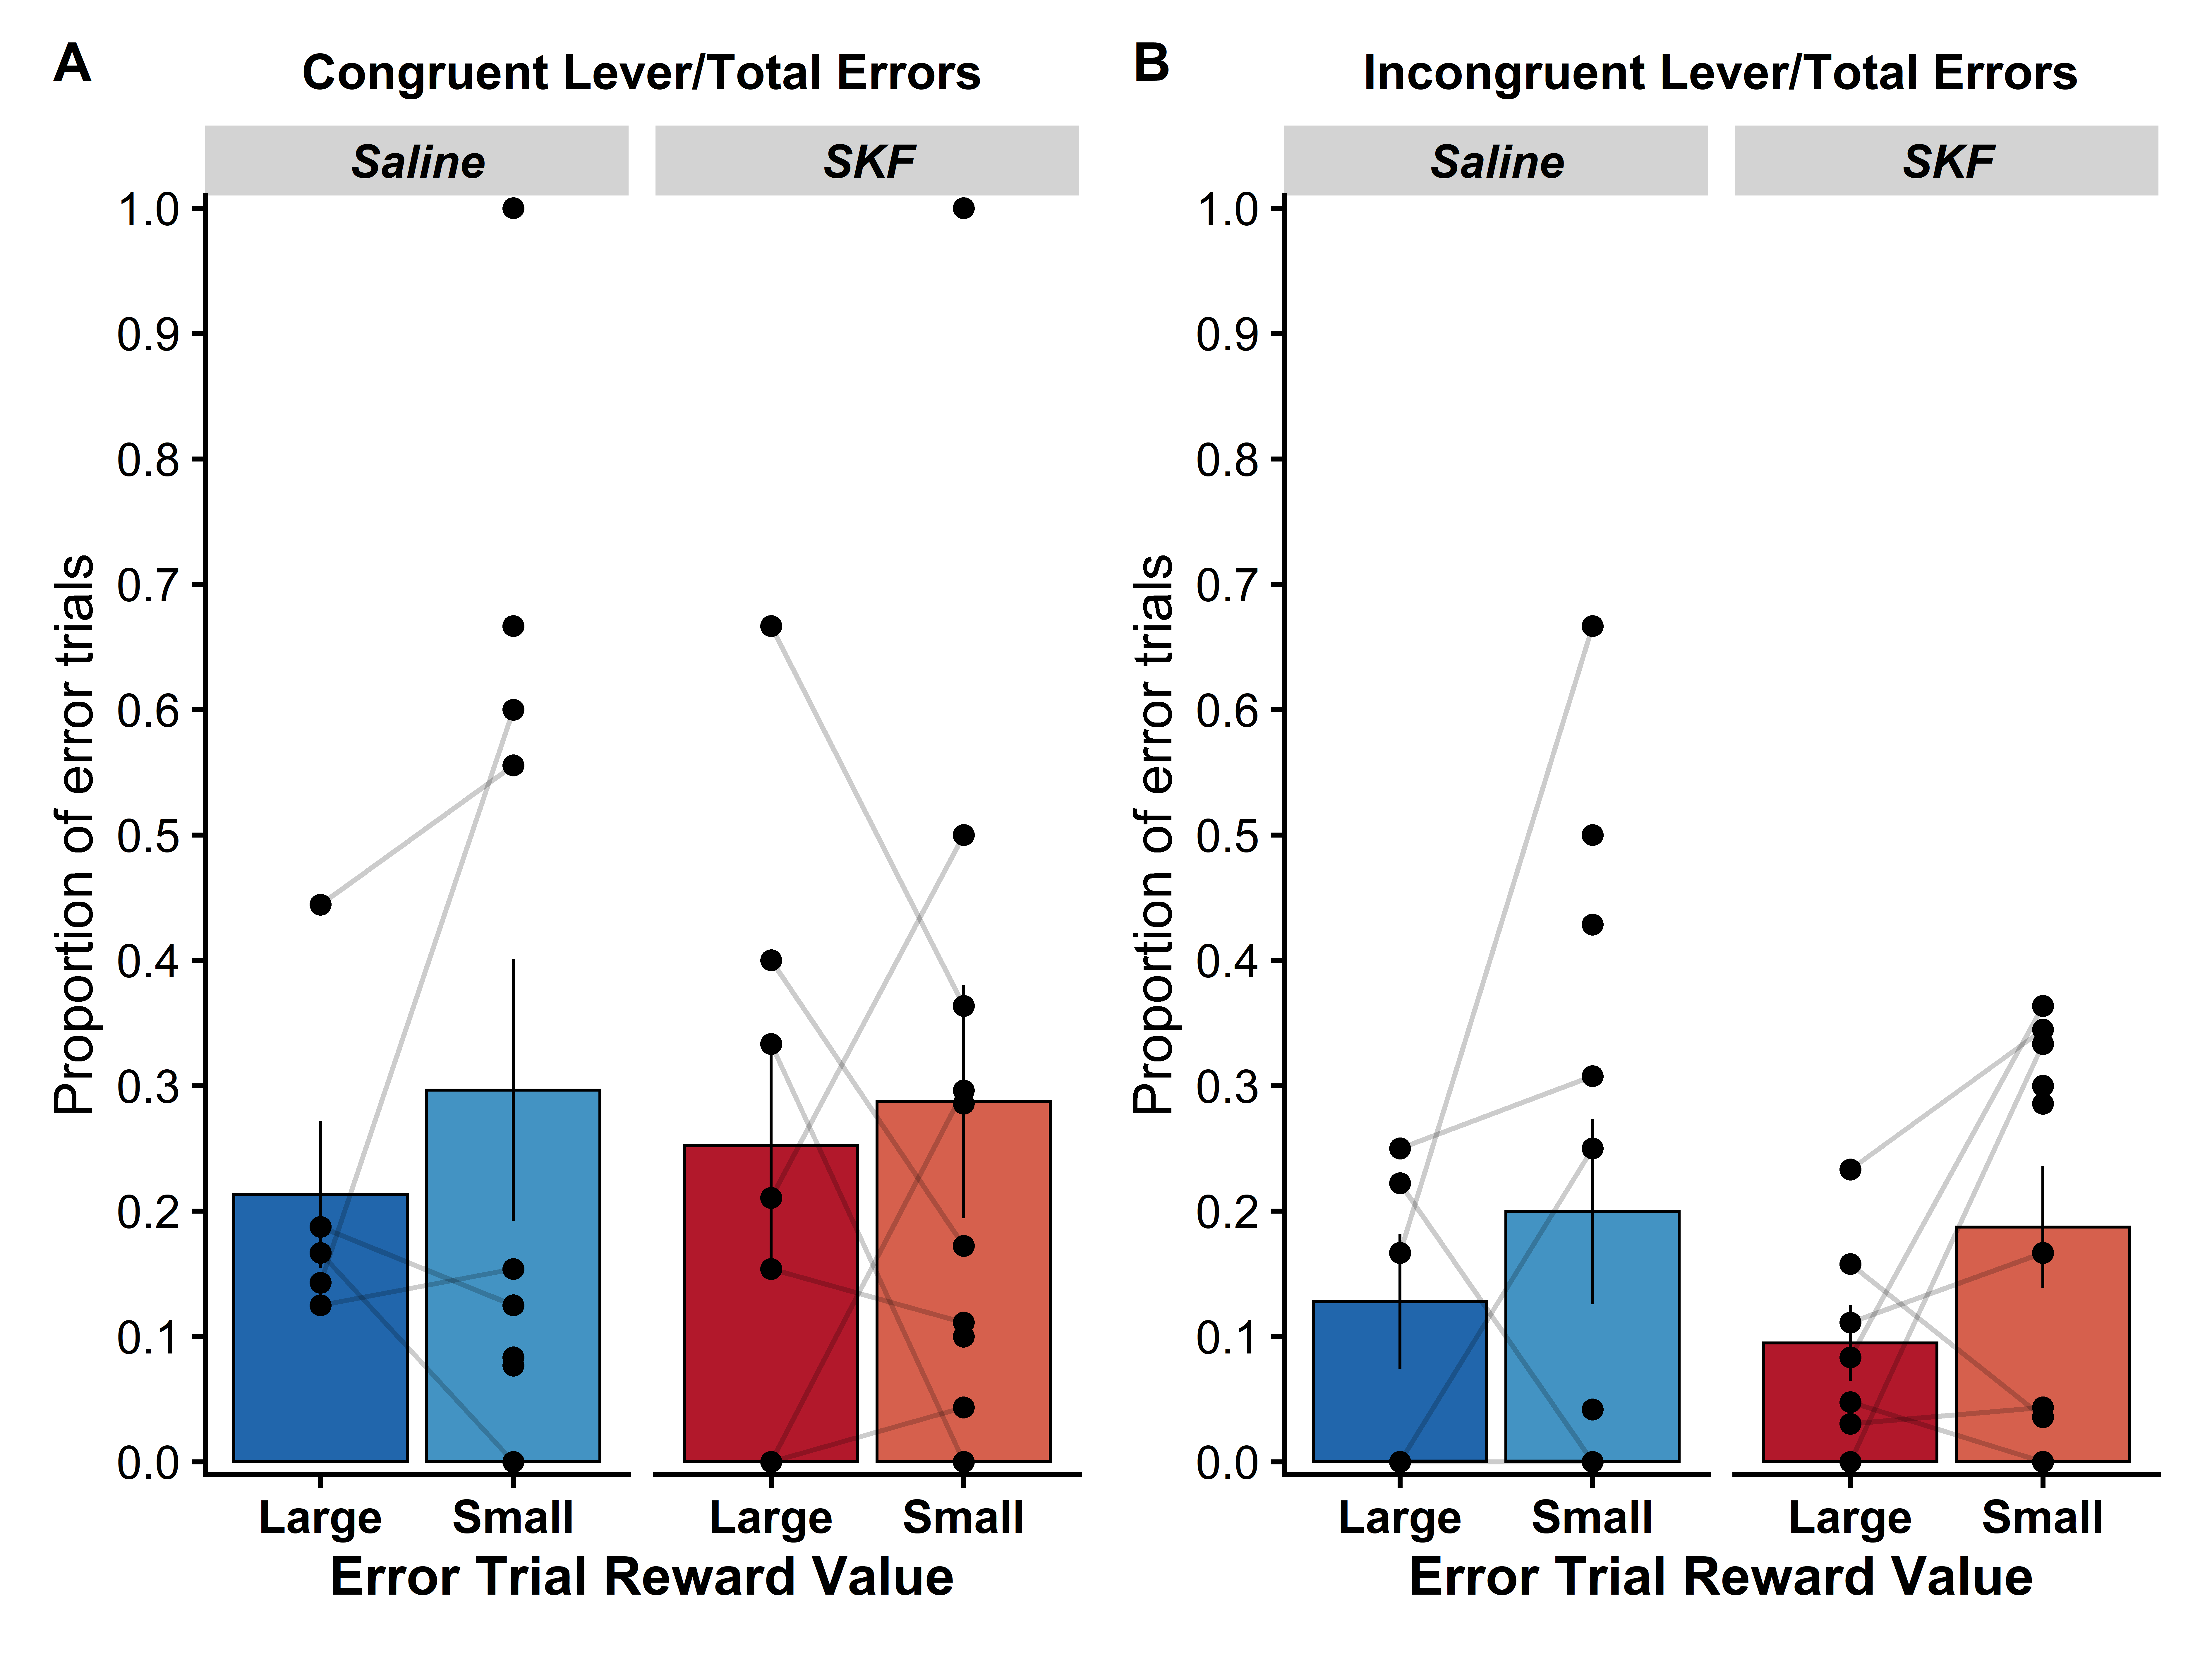
\includegraphics{../figures/Plots_CongruentVsIncongruent.png}
\caption{Probability of congruent and incongruent reward levers}
\end{figure}

\hypertarget{a-analysis-of-congruent-reward-lever}{%
\subsection{A) Analysis of congruent reward
lever}\label{a-analysis-of-congruent-reward-lever}}

\begin{table}[tbp]

\begin{center}
\begin{threeparttable}

\caption{\label{tab:Analysis 2: Probability of both levers }}

\begin{tabular}{lllll}
\toprule
 & \multicolumn{1}{c}{Df} & \multicolumn{1}{c}{Chisq} & \multicolumn{1}{c}{Chi Df} & \multicolumn{1}{c}{Pr(>Chisq)}\\
\midrule
RewardSize & 9.00 & 2.81 & 1.00 & 0.09\\
Drug & 9.00 & 2.89 & 1.00 & 0.09\\
RewardSize:Drug & 9.00 & 0.38 & 1.00 & 0.54\\
\bottomrule
\end{tabular}

\end{threeparttable}
\end{center}

\end{table}

\hypertarget{a-analysis-of-incongruent-reward-lever}{%
\subsection{A) Analysis of incongruent reward
lever}\label{a-analysis-of-incongruent-reward-lever}}

\begin{table}[tbp]

\begin{center}
\begin{threeparttable}

\caption{\label{tab:Analysis 2: Probability of both levers }}

\begin{tabular}{lllll}
\toprule
 & \multicolumn{1}{c}{Df} & \multicolumn{1}{c}{Chisq} & \multicolumn{1}{c}{Chi Df} & \multicolumn{1}{c}{Pr(>Chisq)}\\
\midrule
RewardSize & 9.00 & 1.48 & 1.00 & 0.22\\
Drug & 9.00 & 0.83 & 1.00 & 0.36\\
RewardSize:Drug & 9.00 & 0.24 & 1.00 & 0.63\\
\bottomrule
\end{tabular}

\end{threeparttable}
\end{center}

\end{table}

\end{document}
